\documentclass[11pt,a4paper]{report}
\usepackage[textwidth=37em,vmargin=30mm]{geometry}
\usepackage{calc,xunicode,amsmath,amssymb,paralist,enumitem,tabu,booktabs,datetime2,xeCJK,xeCJKfntef,listings}
\usepackage{tocloft,fancyhdr,tcolorbox,xcolor,graphicx,eso-pic,xltxtra,xelatexemoji}

\newcommand{\envyear}[0]{2025}
\newcommand{\envdatestr}[0]{2025-03-09}
\newcommand{\envfinaldir}[0]{webdb/2025/20250309/final}

\usepackage[hidelinks]{hyperref}
\hypersetup{
    colorlinks=false,
    pdfpagemode=FullScreen,
    pdftitle={Web Digest - \envdatestr}
}

\setlength{\cftbeforechapskip}{10pt}
\renewcommand{\cftchapfont}{\rmfamily\bfseries\large\raggedright}
\setlength{\cftbeforesecskip}{2pt}
\renewcommand{\cftsecfont}{\sffamily\small\raggedright}

\setdefaultleftmargin{2em}{2em}{1em}{1em}{1em}{1em}

\usepackage{xeCJK,xeCJKfntef}
\xeCJKsetup{PunctStyle=plain,RubberPunctSkip=false,CJKglue=\strut\hskip 0pt plus 0.1em minus 0.05em,CJKecglue=\strut\hskip 0.22em plus 0.2em}
\XeTeXlinebreaklocale "zh"
\XeTeXlinebreakskip = 0pt


\setmainfont{Brygada 1918}
\setromanfont{Brygada 1918}
\setsansfont{IBM Plex Sans}
\setmonofont{JetBrains Mono NL}
\setCJKmainfont{Noto Serif CJK SC}
\setCJKromanfont{Noto Serif CJK SC}
\setCJKsansfont{Noto Sans CJK SC}
\setCJKmonofont{Noto Sans CJK SC}

\setlength{\parindent}{0pt}
\setlength{\parskip}{8pt}
\linespread{1.15}

\lstset{
	basicstyle=\ttfamily\footnotesize,
	numbersep=5pt,
	backgroundcolor=\color{black!5},
	showspaces=false,
	showstringspaces=false,
	showtabs=false,
	tabsize=2,
	captionpos=b,
	breaklines=true,
	breakatwhitespace=true,
	breakautoindent=true,
	linewidth=\textwidth
}






\newcommand{\coverpic}[2]{
    % argv: itemurl, authorname
    Cover photo by #2~~(\href{#1}{#1})
}
\newcommand{\makeheader}[0]{
    \begin{titlepage}
        % \newgeometry{hmargin=15mm,tmargin=21mm,bmargin=12mm}
        \begin{center}
            
            \rmfamily\scshape
            \fontspec{BaskervilleF}
            \fontspec{Old Standard}
            \fontsize{59pt}{70pt}\selectfont
            WEB\hfill DIGEST
            
            \vfill
            % \vskip 30pt
            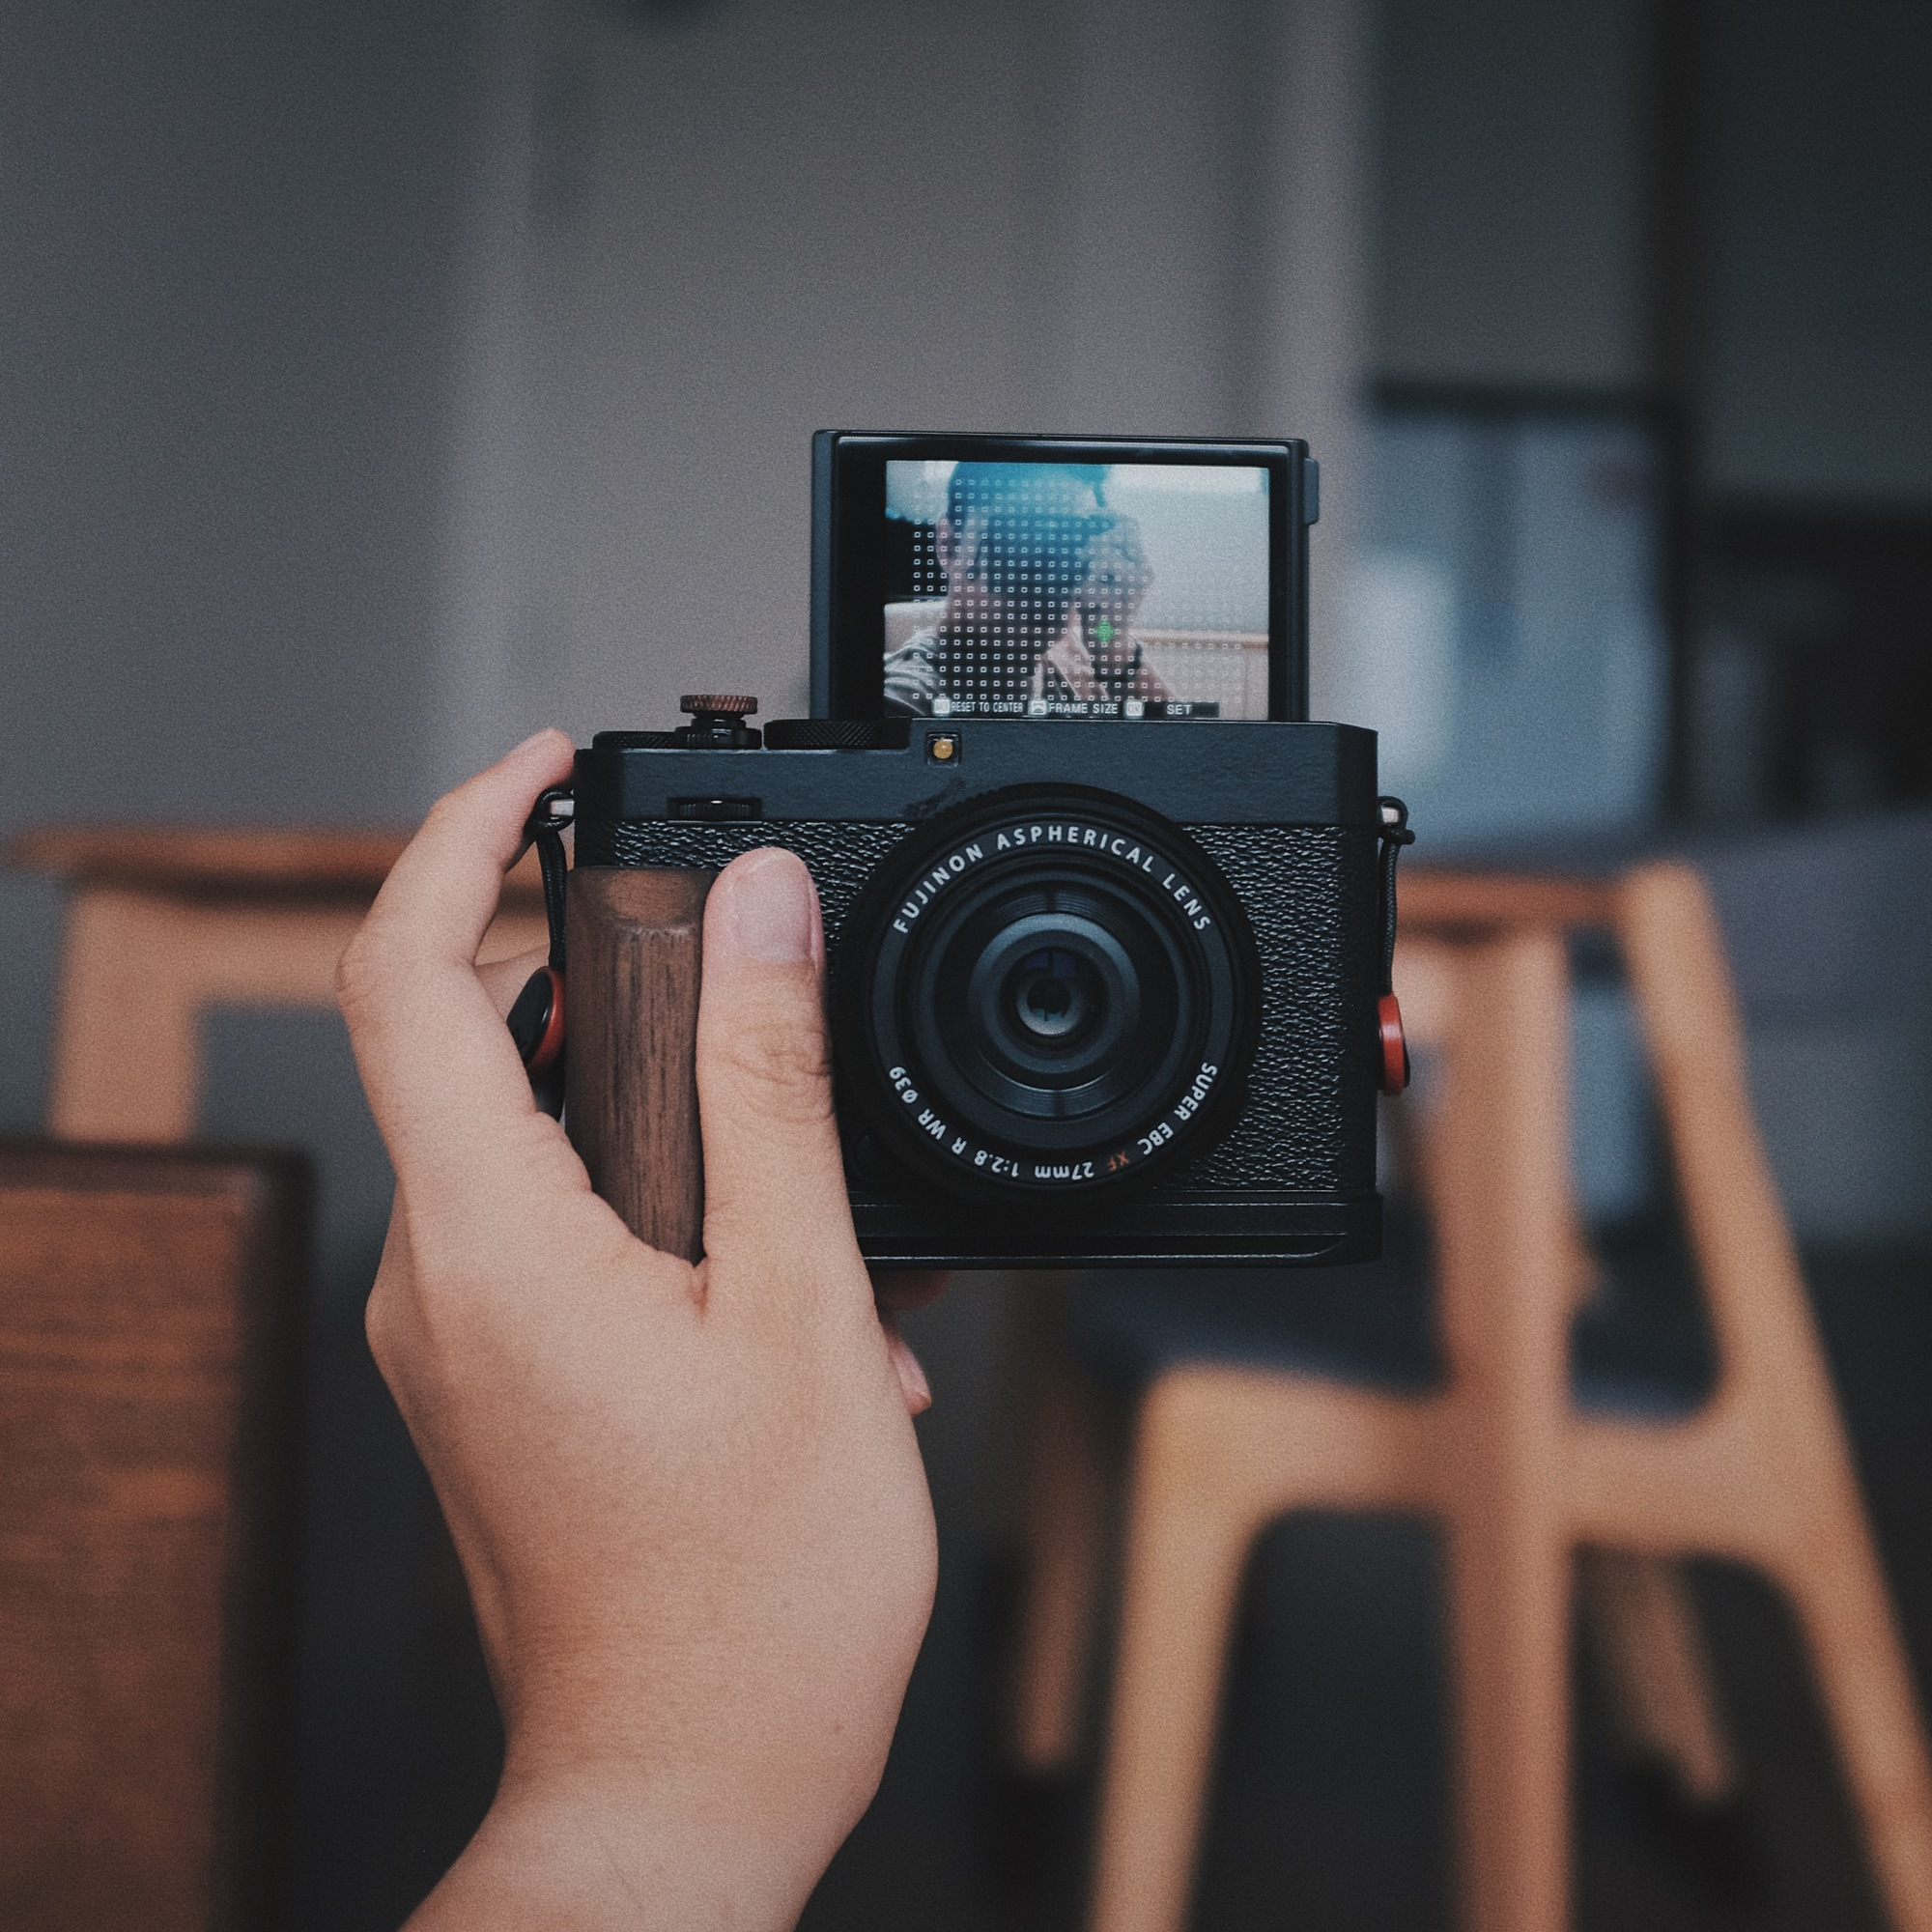
\includegraphics[width=\linewidth]{\envfinaldir/coverpic-prod.jpg}\par
            % \vskip 30pt
            \vfill

            \normalsize\rmfamily\scshape
            \copyright{} The Web Digest Project \hfill\large \envdatestr
        \end{center}
    \end{titlepage}
    % \restoregeometry
}
\newcommand{\simplehref}[1]{%
    \textcolor{blue!80!green}{\href{#1}{#1}}%
}
\renewcommand{\contentsname}{\center\Huge\sffamily\bfseries Contents\par\vskip 20pt}
\newcounter{ipartcounter}
\setcounter{ipartcounter}{0}
\newcommand{\ipart}[1]{
    % \vskip 20pt
    \clearpage
    \stepcounter{ipartcounter}
    \phantomsection
    \addcontentsline{toc}{chapter}{#1}
    % \begin{center}
    %     \Huge
    %     \sffamily\bfseries
    %     #1
    % \end{center}
    % \vskip 20pt plus 7pt
}
\newcounter{ichaptercounter}
\setcounter{ichaptercounter}{0}
\newcommand{\ichapter}[1]{
    % \vskip 20pt
    \clearpage
    \stepcounter{ichaptercounter}
    \phantomsection
    \addcontentsline{toc}{section}{\numberline{\arabic{ichaptercounter}}#1}
    \begin{center}
        \Huge
        \sffamily\bfseries
        #1
    \end{center}
    \vskip 20pt plus 7pt
}
\newcommand{\entrytitlefont}[1]{\subsection*{\raggedright\Large\sffamily\bfseries#1}}
\newcommand{\entryitemGeneric}[2]{
    % argv: title, url
    \parbox{\linewidth}{
        \entrytitlefont{#1}\par\vskip 5pt
        \footnotesize\ttfamily\mdseries
        \simplehref{#2}
    }\vskip 11pt plus 11pt minus 1pt
}
\newcommand{\entryitemGithub}[3]{
    % argv: title, url, desc
    \parbox{\linewidth}{
        \entrytitlefont{#1}\par\vskip 5pt
        \footnotesize\ttfamily\mdseries
        \simplehref{#2}\par\vskip 5pt
        \small\rmfamily\mdseries#3
    }\vskip 11pt plus 11pt minus 1pt
}
\newcommand{\entryitemAp}[3]{
    % argv: title, url, desc
    \parbox{\linewidth}{
        \entrytitlefont{#1}\par\vskip 5pt
        \footnotesize\ttfamily\mdseries
        \simplehref{#2}\par\vskip 5pt
        \small\rmfamily\mdseries#3
    }\vskip 11pt plus 11pt minus 1pt
}
\newcommand{\entryitemHackernews}[3]{
    % argv: title, hnurl, rawurl
    % \parbox{\linewidth}{
    %     \entrytitlefont{#1}\par\vskip 5pt
    %     \footnotesize\ttfamily\mdseries
    %     \simplehref{#3}\par
    %     \textcolor{black!50}{\href{#2}{#2}}
    % }\vskip 11pt plus 11pt minus 1pt
    \begin{minipage}{\linewidth}
            \entrytitlefont{#1}\par\vskip 5pt
            \footnotesize\ttfamily\mdseries
            \simplehref{#3}\par
            \textcolor{black!50}{\href{#2}{#2}}
    \end{minipage}\par\vskip 11pt plus 11pt minus 1pt
}







\begin{document}

\makeheader

\tableofcontents\clearpage




\ipart{Developers}
\ichapter{Hacker News}
\entryitemTwoLinks{Kill your Feeds – Stop letting algorithms dictate what you think}{https://news.ycombinator.com/item?id=43302132}{https://usher.dev/posts/2025-03-08-kill-your-feeds/}

\entryitemTwoLinks{Google will still have to break up its business, the Justice Department said}{https://news.ycombinator.com/item?id=43302097}{https://www.engadget.com/big-tech/google-will-still-have-to-break-up-its-business-the-justice-department-said-150000739.html}

\entryitemTwoLinks{Kagi Is Bringing Orion Web Browser to Linux}{https://news.ycombinator.com/item?id=43302073}{https://www.omgubuntu.co.uk/2025/03/kag-orion-web-browser-coming-to-linux}

\entryitemTwoLinks{Sam Bankman-Fried thrown into solitary over Tucker Carlson interview: report}{https://news.ycombinator.com/item?id=43301702}{https://gizmodo.com/sam-bankman-fried-thrown-into-solitary-over-tucker-carlson-interview-report-2000573371}

\entryitemTwoLinks{You might not need Redis}{https://news.ycombinator.com/item?id=43301432}{https://www.viblo.se/posts/no-need-redis/}

\entryitemTwoLinks{Undocumented backdoor found in Bluetooth chip used by a billion devices}{https://news.ycombinator.com/item?id=43301369}{https://www.bleepingcomputer.com/news/security/undocumented-backdoor-found-in-bluetooth-chip-used-by-a-billion-devices/}

\entryitemTwoLinks{Discovering errors in Donald Knuth's TAOCP}{https://news.ycombinator.com/item?id=43301342}{https://glthr.com/discovering-errors-in-donald-knuths-taocp}

\entryitemTwoLinks{The program is the database is the interface}{https://news.ycombinator.com/item?id=43300528}{https://www.scattered-thoughts.net/writing/the-program-is-the-database-is-the-interface/}

\entryitemTwoLinks{The DOJ still wants Google to sell off Chrome}{https://news.ycombinator.com/item?id=43299886}{https://www.wired.com/story/the-doj-still-wants-google-to-divest-chrome/}

\entryitemTwoLinks{Discworld Rules}{https://news.ycombinator.com/item?id=43299815}{https://contraptions.venkateshrao.com/p/discworld-rules}

\entryitemTwoLinks{Volkswagen reintroducing physical controls for vital functions}{https://news.ycombinator.com/item?id=43298271}{https://www.autocar.co.uk/car-news/new-cars/volkswagen-reintroducing-physical-controls-vital-functions}

\entryitemTwoLinks{PayPal honey extension has again "featured" flag in Chrome web store}{https://news.ycombinator.com/item?id=43298054}{https://chromewebstore.google.com/detail/paypal-honey-automatic-co/bmnlcjabgnpnenekpadlanbbkooimhnj/reviews}

\entryitemTwoLinks{Falkon: A KDE Web Browser}{https://news.ycombinator.com/item?id=43297590}{https://www.falkon.org}

\entryitemTwoLinks{An epic treatise on error models for systems programming languages}{https://news.ycombinator.com/item?id=43297574}{https://typesanitizer.com/blog/errors.html}

\entryitemTwoLinks{Show HN: Open-Source DocumentAI with Ollama}{https://news.ycombinator.com/item?id=43296918}{https://rlama.dev/}

\entryitemTwoLinks{Take It Down Act: A Flawed Attempt to Protect Victims That'll Lead to Censorship}{https://news.ycombinator.com/item?id=43296886}{https://www.eff.org/deeplinks/2025/02/take-it-down-act-flawed-attempt-protect-victims-will-lead-censorship}

\entryitemTwoLinks{Feds Link Cyberheist to 2022 LastPass Hacks}{https://news.ycombinator.com/item?id=43296656}{https://krebsonsecurity.com/2025/03/feds-link-150m-cyberheist-to-2022-lastpass-hacks/}

\entryitemTwoLinks{GeoCities in 1995: Building a Home Page on the Internet}{https://news.ycombinator.com/item?id=43296103}{https://cybercultural.com/p/geocities-1995/}

\entryitemTwoLinks{How did places like Bell Labs know how to ask the right questions? (2023)}{https://news.ycombinator.com/item?id=43295865}{https://www.freaktakes.com/p/how-did-places-like-bell-labs-know}

\entryitemTwoLinks{AI tools are spotting errors in research papers}{https://news.ycombinator.com/item?id=43295692}{https://www.nature.com/articles/d41586-025-00648-5}\ichapter{Phoronix}
\entryitemGeneric{\hskip 0pt{}Wine Releases Framework Mono 6.14 In Taking Over The Mono Project}{https://www.phoronix.com/news/Wine-Framework-Mono-6.14}

\entryitemGeneric{\hskip 0pt{}Rust Coreutils 0.0.30 Enhances GNU Compatibility, Uutils To Port More Common Unix Tools}{https://www.phoronix.com/news/uutils-Coreutils-0.0.30}

\entryitemGeneric{\hskip 0pt{}GTK On Android \& macOS Seeing Improvements}{https://www.phoronix.com/news/GNOME-GTK-Android-macOS}

\entryitemGeneric{\hskip 0pt{}Mesa's Venus Driver Adds Vulkan Ray-Tracing Support For VMs}{https://www.phoronix.com/news/Mesa-25.1-Venus-Vulkan-RT}

\entryitemGeneric{\hskip 0pt{}Wine-Staging 10.3 Adds Patch For A 15 Year Old Bug}{https://www.phoronix.com/news/Wine-Staging-10.3}

\entryitemGeneric{\hskip 0pt{}KDE This Week Took Care Of "A Very Large Number Of Bugs"}{https://www.phoronix.com/news/KDE-Fixes-Large-Num-Bugs}

\entryitemGeneric{\hskip 0pt{}Wine 10.3 Wires Up Wayland Driver Clipboard Handling, Vulkan Video Decode Within WineD3D}{https://www.phoronix.com/news/Wine-10.3-Released}

\entryitemGeneric{\hskip 0pt{}GNOME 48 Release Candidate Brings Late Mutter Features \& Other Changes}{https://www.phoronix.com/news/GNOME-48-Release-Candidate}

\entryitemGeneric{\hskip 0pt{}Vulkan Video Continues Making Inroads, VP9 Decode Planned For This Year}{https://www.phoronix.com/news/Vulkan-Video-2025-Plans}\ichapter{Dribbble}
\entryitemGeneric{\hskip 0pt{}Free Fly Apparel}{https://dribbble.com/shots/25727838-Free-Fly-Apparel}

\entryitemGeneric{\hskip 0pt{}Columbus Rapids® C-Wave}{https://dribbble.com/shots/25727535-Columbus-Rapids-C-Wave}

\entryitemGeneric{\hskip 0pt{}Bloodhound Detective}{https://dribbble.com/shots/25726401-Bloodhound-Detective}

\entryitemGeneric{\hskip 0pt{}QLOUD - Logo Redesign}{https://dribbble.com/shots/25726630-QLOUD-Logo-Redesign}

\entryitemGeneric{\hskip 0pt{}Chief Logo and Branding Identity}{https://dribbble.com/shots/25723018-Chief-Logo-and-Branding-Identity}

\entryitemGeneric{\hskip 0pt{}Logo Design for Streaming Platform (Unused for Sale)}{https://dribbble.com/shots/25726051-Logo-Design-for-Streaming-Platform-Unused-for-Sale}

\entryitemGeneric{\hskip 0pt{}Puzzle Fintech Website Design}{https://dribbble.com/shots/25651990-Puzzle-Fintech-Website-Design}

\entryitemGeneric{\hskip 0pt{}Dashboard for an Education Product ✦ Golf Pro}{https://dribbble.com/shots/25720487-Dashboard-for-an-Education-Product-Golf-Pro}

\entryitemGeneric{\hskip 0pt{}Proboscis Monkey}{https://dribbble.com/shots/25720978-Proboscis-Monkey}

\entryitemGeneric{\hskip 0pt{}Logofolio Update - March 2025}{https://dribbble.com/shots/25719985-Logofolio-Update-March-2025}

\entryitemGeneric{\hskip 0pt{}Bento grid barbershop platform UI}{https://dribbble.com/shots/25715947-Bento-grid-barbershop-platform-UI}

\entryitemGeneric{\hskip 0pt{}Cimet Slogan}{https://dribbble.com/shots/25710581-Cimet-Slogan}

\entryitemGeneric{\hskip 0pt{}FUUL // Branding Identity}{https://dribbble.com/shots/25719928-FUUL-Branding-Identity}

\entryitemGeneric{\hskip 0pt{}Real Estate Platform UI}{https://dribbble.com/shots/25711538-Real-Estate-Platform-UI}

\entryitemGeneric{\hskip 0pt{}Easy A Deck}{https://dribbble.com/shots/25715917-Easy-A-Deck}

\entryitemGeneric{\hskip 0pt{}Letter C + Hummingbird}{https://dribbble.com/shots/25713900-Letter-C-Hummingbird}

\entryitemGeneric{\hskip 0pt{}Logistics Company Web Design Landing Page}{https://dribbble.com/shots/25708252-Logistics-Company-Web-Design-Landing-Page}

\entryitemGeneric{\hskip 0pt{}Inner Truth}{https://dribbble.com/shots/25659901-Inner-Truth}

\entryitemGeneric{\hskip 0pt{}Landing Page: AI Testing}{https://dribbble.com/shots/25714074-Landing-Page-AI-Testing}

\entryitemGeneric{\hskip 0pt{}Star + Check Mark Icon Concept}{https://dribbble.com/shots/25709690-Star-Check-Mark-Icon-Concept}

\entryitemGeneric{\hskip 0pt{}FREELANCE (Finally)}{https://dribbble.com/shots/25710537-FREELANCE-Finally}

\entryitemGeneric{\hskip 0pt{}Recent Logo Designs - Jeroen van Eerden}{https://dribbble.com/shots/25709914-Recent-Logo-Designs-Jeroen-van-Eerden}

\entryitemGeneric{\hskip 0pt{}Wolf}{https://dribbble.com/shots/25707625-Wolf}

\entryitemGeneric{\hskip 0pt{}Boletus logo}{https://dribbble.com/shots/25709349-Boletus-logo}


\ipart{Developers~~~~(zh-Hans)}
\ichapter{Solidot}
\entryitemGeneric{\hskip 0pt{}印度女性每天在无偿家务上的时间两倍多于男性}{https://www.solidot.org/story?sid=80738}

\entryitemGeneric{\hskip 0pt{}巴西法官命令苹果在 90 天内开放其 iOS 平台}{https://www.solidot.org/story?sid=80737}

\entryitemGeneric{\hskip 0pt{}微软开发与 OpenAI 竞争的大模型 MAI}{https://www.solidot.org/story?sid=80736}

\entryitemGeneric{\hskip 0pt{}柯伊伯带可能有很多三体系统}{https://www.solidot.org/story?sid=80735}

\entryitemGeneric{\hskip 0pt{}Intuitive Machines 的雅典娜月球探测器因侧翻而提前终止任务}{https://www.solidot.org/story?sid=80734}

\entryitemGeneric{\hskip 0pt{}天文学家认为一颗垂死恒星发出的神秘信号源自被撕裂的行星}{https://www.solidot.org/story?sid=80733}

\entryitemGeneric{\hskip 0pt{}周末前做手术有更高的死亡和并发症风险}{https://www.solidot.org/story?sid=80732}

\entryitemGeneric{\hskip 0pt{}研究人员从拉布拉多身上发现人犬共享肥胖相关基因}{https://www.solidot.org/story?sid=80731}

\entryitemGeneric{\hskip 0pt{}Google 以国家安全理由希望不被肢解}{https://www.solidot.org/story?sid=80730}

\entryitemGeneric{\hskip 0pt{}光首次被转化为超固体}{https://www.solidot.org/story?sid=80729}

\entryitemGeneric{\hskip 0pt{}NASA 关闭航海家的科学设备以节省电力}{https://www.solidot.org/story?sid=80728}

\entryitemGeneric{\hskip 0pt{}研究发现精液质量与男性寿命相关}{https://www.solidot.org/story?sid=80727}

\entryitemGeneric{\hskip 0pt{}NASA 首次在月球上使用 GPS }{https://www.solidot.org/story?sid=80726}

\entryitemGeneric{\hskip 0pt{}OpenAI 计划对博士水平的 AI 智能体收取 2 万美元月费}{https://www.solidot.org/story?sid=80725}

\entryitemGeneric{\hskip 0pt{}36 家石化巨头产生的碳排放占到了全球的一半}{https://www.solidot.org/story?sid=80724}

\entryitemGeneric{\hskip 0pt{}美国停止分享大使馆领事馆收集的空气质量数据}{https://www.solidot.org/story?sid=80723}

\entryitemGeneric{\hskip 0pt{}全球暖化威胁低纬度地区到粮食产量}{https://www.solidot.org/story?sid=80722}

\entryitemGeneric{\hskip 0pt{}犹他州要求美国应用商店验证用户年龄}{https://www.solidot.org/story?sid=80721}\ichapter{V2EX}
\entryitemGeneric{\hskip 0pt{}[Windows] 突然发现 WSL 支持安装发行版时自定义名称了(相同发行版可共存)}{https://www.v2ex.com/t/1116987}

\entryitemGeneric{\hskip 0pt{}[Chrome] MacOS 中如何彻底禁止 Chrome 更新}{https://www.v2ex.com/t/1116985}

\entryitemGeneric{\hskip 0pt{}[分享创造] 用 claude3.7 做的一个小游戏站点}{https://www.v2ex.com/t/1116984}

\entryitemGeneric{\hskip 0pt{}[问与答] 有什么离线的去除图片杂物的方案}{https://www.v2ex.com/t/1116983}

\entryitemGeneric{\hskip 0pt{}[酷工作] 阿里云-MaxCompute Data + AI 计算框架团队招聘研发 P6-P8 同学-杭州/北京}{https://www.v2ex.com/t/1116977}

\entryitemGeneric{\hskip 0pt{}[Apple] 请教用过苹果 ai 的}{https://www.v2ex.com/t/1116976}

\entryitemGeneric{\hskip 0pt{}[分享创造] [旅行 APP 产品诞生日记] 11day/100days}{https://www.v2ex.com/t/1116974}

\entryitemGeneric{\hskip 0pt{}[全球工单系统] B 站又又又又崩了??}{https://www.v2ex.com/t/1116973}

\entryitemGeneric{\hskip 0pt{}[全球工单系统] B 站首页挂了?}{https://www.v2ex.com/t/1116972}

\entryitemGeneric{\hskip 0pt{}[硬件] 2.5 寸机械移动硬盘在桌面上滑动,对硬盘危险么?该怎么防护?}{https://www.v2ex.com/t/1116971}

\entryitemGeneric{\hskip 0pt{}[问与答] 有什么能提升幸福感的软装物件推荐吗}{https://www.v2ex.com/t/1116970}

\entryitemGeneric{\hskip 0pt{}[问与答] 求推荐 esim 保号卡}{https://www.v2ex.com/t/1116969}

\entryitemGeneric{\hskip 0pt{}[酷工作] [北京-WLB 外企 A 轮] 招聘前后端研发工程师, SaaS 产品经理,设计师}{https://www.v2ex.com/t/1116968}

\entryitemGeneric{\hskip 0pt{}[求职] 互联网工作求助(或者在日工作的)}{https://www.v2ex.com/t/1116967}

\entryitemGeneric{\hskip 0pt{}[程序员] Manus AI 是否真的像宣传的那么回事?}{https://www.v2ex.com/t/1116963}

\entryitemGeneric{\hskip 0pt{}[宽带症候群] 用着广东电信宽带的朋友们,你们的 IPv6 网络正常吗?}{https://www.v2ex.com/t/1116962}

\entryitemGeneric{\hskip 0pt{}[问与答] 可以推荐点可以调用大模型和网页对话的浏览器插件吗?}{https://www.v2ex.com/t/1116961}

\entryitemGeneric{\hskip 0pt{}[奇思妙想] 小米手环当钥匙扣门牌}{https://www.v2ex.com/t/1116960}

\entryitemGeneric{\hskip 0pt{}[宽带症候群] 移动换着花样阻止我上传,给我气笑了}{https://www.v2ex.com/t/1116959}

\entryitemGeneric{\hskip 0pt{}[程序员] 现在来看, C/C++ 的 int、long 等不定宽类型是失败的设计吗?}{https://www.v2ex.com/t/1116958}

\entryitemGeneric{\hskip 0pt{}[浏览器] 大家的 Chrome 浏览器有哪些推荐的插件呢?}{https://www.v2ex.com/t/1116957}

\entryitemGeneric{\hskip 0pt{}[推广] 最近港股有点猛,给兄弟们推荐一个最便宜的港股券商,有 AFF}{https://www.v2ex.com/t/1116954}

\entryitemGeneric{\hskip 0pt{}[云计算] AWS 多可用区下的服务发现架构产生的流量问题}{https://www.v2ex.com/t/1116951}

\entryitemGeneric{\hskip 0pt{}[问与答] ikuai 中的虚拟机总是无端死机,无法访问}{https://www.v2ex.com/t/1116950}

\entryitemGeneric{\hskip 0pt{}[问与答] mac mini 挂外接硬盘。一步到位还是够用就行。}{https://www.v2ex.com/t/1116949}

\entryitemGeneric{\hskip 0pt{}[问与答] 显示器 DELL U3225QE 和 LG 32gq950、32GS95UE 怎么选?}{https://www.v2ex.com/t/1116948}

\entryitemGeneric{\hskip 0pt{}[微信] 语音和视频用系统电话接通, Apple Watch 来电不提醒}{https://www.v2ex.com/t/1116947}

\entryitemGeneric{\hskip 0pt{}[分享创造] AI Chat Session Navigator 一个为你的 ChatGPT/Deepseek/Poe 提升使用效率的工具}{https://www.v2ex.com/t/1116946}

\entryitemGeneric{\hskip 0pt{}[分享发现] 国内头部的云服务器厂商,企业折扣你们能拿到多少?(8 折的算是普通)}{https://www.v2ex.com/t/1116944}

\entryitemGeneric{\hskip 0pt{}[Linux] 跟着 ChatGPT 捣鼓 CasaOS 把群晖文件全删光了}{https://www.v2ex.com/t/1116943}

\entryitemGeneric{\hskip 0pt{}[分享发现] 整理了一些生活好物+数码产品分享,大家也可以分享一下你们觉得好用的物品}{https://www.v2ex.com/t/1116942}

\entryitemGeneric{\hskip 0pt{}[NAS] NAS 积满灰尘, 怎么清理?}{https://www.v2ex.com/t/1116941}

\entryitemGeneric{\hskip 0pt{}[问与答] 中国移动的``达量限速''是不是约等于无限流量?}{https://www.v2ex.com/t/1116938}

\entryitemGeneric{\hskip 0pt{}[酷工作] [广州-三七互娱-社招内推] 中级、高级、资深 Golang 后端开发工程师}{https://www.v2ex.com/t/1116937}

\entryitemGeneric{\hskip 0pt{}[程序员] 推荐个便携显示器吧}{https://www.v2ex.com/t/1116936}

\entryitemGeneric{\hskip 0pt{}[Telegram] telegram 的 web 版, F12 里完全看不到网络请求,这是用了什么黑科技?}{https://www.v2ex.com/t/1116935}

\entryitemGeneric{\hskip 0pt{}[问与答] Apple Mini M4 + Dell 2K 显示器经常黑屏闪烁}{https://www.v2ex.com/t/1116933}

\entryitemGeneric{\hskip 0pt{}[路由器] 中兴 BE5100Pro+和小米 BE6500 标准版怎么选?巡天和晴天呢?}{https://www.v2ex.com/t/1116932}

\entryitemGeneric{\hskip 0pt{}[业界八卦] 将来某一天,雷军会不会塌方?现在很多喊雷爸爸的正如当年很多喊马爸爸的🤔}{https://www.v2ex.com/t/1116931}

\entryitemGeneric{\hskip 0pt{}[iOS] 在 11 寸的 iPad 上如何优雅使用 Office 文件}{https://www.v2ex.com/t/1116930}

\entryitemGeneric{\hskip 0pt{}[NAS] 这是群晖的问题还是外挂硬盘盒的问题}{https://www.v2ex.com/t/1116929}

\entryitemGeneric{\hskip 0pt{}[问与答] 低成本 GPT PLUS 是怎么开通的?}{https://www.v2ex.com/t/1116928}

\entryitemGeneric{\hskip 0pt{}[分享创造] 我用邮件做了一个 RSS 订阅源}{https://www.v2ex.com/t/1116927}

\entryitemGeneric{\hskip 0pt{}[分享创造] 有人愿意来帮忙指点一下我做的一个 AI agent 吗(已开源)}{https://www.v2ex.com/t/1116926}

\entryitemGeneric{\hskip 0pt{}[问与答] 我的一个 prompt,在 DeepSeek 上答案都不同,晕了}{https://www.v2ex.com/t/1116925}

\entryitemGeneric{\hskip 0pt{}[分享创造] 中英文完美 2:1 宽的 JetBrains Maple Mono 开源合成字体 [工整,优雅,超高可读性]}{https://www.v2ex.com/t/1116924}

\entryitemGeneric{\hskip 0pt{}[优惠信息] u2725qe 并夕夕 补贴后 4k(3999)}{https://www.v2ex.com/t/1116923}

\entryitemGeneric{\hskip 0pt{}[NAS] 百度网盘还真不要脸,造假显示速率}{https://www.v2ex.com/t/1116922}

\entryitemGeneric{\hskip 0pt{}[问与答] 好像刚上的双影奇境未包含在 EA Play 里...}{https://www.v2ex.com/t/1116921}

\entryitemGeneric{\hskip 0pt{}[Apple] 求一个可以对文本执行查找和替换操作的 App}{https://www.v2ex.com/t/1116920}


\ipart{Generic News}
\ichapter{AP News}
\entryitemWithDescription{\hskip 0pt{}A man with a Palestinian flag climbs London's Big Ben tower and refuses to come down}{https://apnews.com/article/78efffa02b2236e85d1693f5a3924af2}{}

\entryitemWithDescription{\hskip 0pt{}Watch the moon turn red during a total lunar eclipse in March}{https://apnews.com/article/97632bddb4896656b3adb7fd6d818562}{}

\entryitemWithDescription{\hskip 0pt{}Chiefs receiver Xavier Worthy is arrested in Texas on a family violence assault charge}{https://apnews.com/article/4d3b3bb4c3608a5be74f2dda420f0044}{}

\entryitemWithDescription{\hskip 0pt{}1 dead and several injured as tropical low tracks west across Australian east coast}{https://apnews.com/article/ec60b6f7b8658e9cdce954c7a47979f1}{}

\entryitemWithDescription{\hskip 0pt{}`With Love, Meghan,' the Duchess of Sussex's Netflix series, renewed for a second season}{https://apnews.com/article/fc4297cc127bd92b618d7a2b4e2d4242}{}

\entryitemWithDescription{\hskip 0pt{}What is hantavirus, the infection that killed Betsy Arakawa, Gene Hackman's wife?}{https://apnews.com/article/af52b4943d854b52a5da36100113bc1b}{}

\entryitemWithDescription{\hskip 0pt{}A car pulled from a river may tell what happened to an Oregon family of 5 that went missing in 1958}{https://apnews.com/article/f836881364b67c816c8883766a75c8c5}{}

\entryitemWithDescription{\hskip 0pt{}US military's mini space shuttle returns to Earth after orbiting for 434 days on a secret mission}{https://apnews.com/article/b62ef48f514dff2a3737afc2e5c241e6}{}

\entryitemWithDescription{\hskip 0pt{}Why are clocks set forward in the spring? Thank wars, confusion and a hunger for sunlight}{https://apnews.com/article/c87a434fb84af044690ad0f48c80544e}{}

\entryitemWithDescription{\hskip 0pt{}Ricardo Scofidio, architect behind New York City's High Line park, dies at 89}{https://apnews.com/article/eb06071fa45b0fdeb462dfc885ae6e5c}{}

\entryitemWithDescription{\hskip 0pt{}This portrait may be the only one of England's 9-day queen painted during her lifetime}{https://apnews.com/article/760d15fa05a579e1e8f5c7836df41d4a}{}

\entryitemWithDescription{\hskip 0pt{}Crews battle fire on 3 yachts in Miami}{https://apnews.com/article/befea696b3d26669d1f8500d83aed360}{}

\entryitemWithDescription{\hskip 0pt{}MLB players' union, Bad Bunny agency agree to dismiss lawsuit over discipline}{https://apnews.com/article/0fdf255a93cab262dcfeaf2b19ea86b0}{}\ichapter{Reuters}
\entryitemWithDescription{\hskip 0pt{}Russian strike on eastern Ukrainian town kills four, injures 18, regional governor says}{https://www.reuters.com/world/europe/russian-strike-eastern-ukrainian-town-kills-four-injures-18-regional-governor-2025-03-07/}{Russian forces attacked the town of Dobropillia in eastern Ukraine late on Friday, killing four people and injuring 18, the regional governor...}

\entryitemWithDescription{\hskip 0pt{}Drugs to blame in Liam Payne's death, close friend says}{https://www.reuters.com/lifestyle/drugs-blame-liam-paynes-death-close-friend-says-2025-03-07/}{Drugs are the only thing to blame in the death of former One Direction star Liam Payne, according to a close friend who was cleared last month of charges he was involved with the singer\textquotesingle s...}

\entryitemWithDescription{\hskip 0pt{}Cyclone Alfred downgraded as millions of Australians stay indoors}{https://www.reuters.com/business/environment/cyclone-alfred-downgraded-millions-australians-stay-indoors-2025-03-07/}{Ex-tropical cyclone Alfred, expected to hit the mainland of east Australia in the next few hours, was downgraded to a \textquotesingle tropical low\textquotesingle{} on Saturday, but officials warn that the storm can still bring severe...}

\entryitemWithDescription{\hskip 0pt{}Women's rights under attack and 'we must fight back', says UN chief}{https://www.reuters.com/world/womens-rights-under-attack-we-must-fight-back-says-un-chief-2025-03-07/}{Women\textquotesingle s rights are under attack and "we must fight back," United Nations Secretary-General Antonio Guterres said on Friday, warning that the world cannot stand by as progress is...}

\entryitemWithDescription{\hskip 0pt{}US State Dept employee arrested on conspiracy charges related to defense information}{https://www.reuters.com/world/us/us-state-dept-employee-arrested-conspiracy-charges-related-defense-information-2025-03-07/}{The U.S. Justice Department said on Friday that a State Department employee was arrested on criminal charges related to alleged participation in a conspiracy to gather, transmit, or lose national defense...}

\entryitemWithDescription{\hskip 0pt{}US foreign aid orgs say they are owed more than \$671 mln by Monday deadline}{https://www.reuters.com/world/us/us-foreign-aid-orgs-say-they-are-owed-more-than-671-mln-by-monday-deadline-2025-03-07/}{U.S. foreign aid organizations suing President Donald Trump\textquotesingle s administration over its freeze of nearly all foreign aid spending said on Friday that they are owed more than \$671 million for past work that a court has...}

\entryitemWithDescription{\hskip 0pt{}Greek government survives confidence vote over deadly 2023 train crash, clashes erupt}{https://www.reuters.com/world/europe/greek-government-survives-confidence-vote-over-deadly-2023-train-crash-clashes-2025-03-07/}{Greece\textquotesingle s centre-right government on Friday survived a no-confidence vote over a deadly 2023 train crash, as protests flared demanding political accountability over Greece\textquotesingle s worst rail...}

\entryitemWithDescription{\hskip 0pt{}Musk, Rubio clash in cabinet meeting, New York Times says}{https://www.reuters.com/world/us/musk-rubio-clash-cabinet-meeting-new-york-times-says-2025-03-07/}{U.S. Secretary of State Marco Rubio and billionaire White House adviser Elon Musk clashed on Thursday during a Cabinet meeting, as President Donald Trump watched, over the level of staff cuts that Rubio has carried out, the New York Times...}

\entryitemWithDescription{\hskip 0pt{}As US restores some aid, humanitarian groups ask: where is the money?}{https://www.reuters.com/business/healthcare-pharmaceuticals/us-restores-some-aid-humanitarian-groups-ask-where-is-money-2025-03-07/}{Days after cutting billions of dollars in foreign aid programs, the United States began reversing some decisions, but humanitarian groups say funds have not yet arrived and the United Nations has started evaluating "choices we are making...}

\entryitemWithDescription{\hskip 0pt{}Haitian economist takes over as transition president in friendly ceremony}{https://www.reuters.com/world/americas/haitian-economist-takes-over-transition-president-friendly-ceremony-2025-03-07/}{Haitian economist and former central bank chief Fritz Alphonse Jean took over the rotating presidency of Haiti\textquotesingle s transitional presidential council on Friday, taking the top executive role in a country battling a...}

\entryitemWithDescription{\hskip 0pt{}Exclusive: US mulls how to ease Russia energy sanctions quickly if war ends, sources say}{https://www.reuters.com/world/us/us-mulls-how-ease-russia-energy-sanctions-quickly-if-war-ends-sources-say-2025-03-07/}{The U.S. government is studying ways it could ease sanctions on Russia\textquotesingle s energy sector as part of a broad plan to enable Washington to deliver swift relief if Moscow agrees to end the Ukraine war, according to two sources...}

\entryitemWithDescription{\hskip 0pt{}Trump threatens Russia with sanctions until Ukraine peace reached}{https://www.reuters.com/world/europe/trump-threatens-russia-with-sanctions-until-ukraine-peace-agreed-2025-03-07/}{U.S. President Donald Trump raised the prospect of imposing large-scale U.S. sanctions on Russia on Friday, days after pausing military aid and intelligence support to Ukraine, and he called on both countries to get on with negotiating a...}

\entryitemWithDescription{\hskip 0pt{}US reciprocal tariffs will impose one rate per country, White House adviser says}{https://www.reuters.com/world/us/us-reciprocal-tariffs-will-impose-one-rate-per-country-white-house-adviser-says-2025-03-07/}{President Donald Trump\textquotesingle s reciprocal tariffs planned for April 2 will impose one rate for each country that will reflect tariffs and non-tariff measures imposed on the U.S., White House trade adviser Peter Navarro told CNBC...}






\clearpage
\leavevmode\vfill
\footnotesize

Copyright \copyright{} 2023-2025 Neruthes and other contributors.

This document is published with CC BY-NC-ND 4.0 license.

The entries listed in this newsletter may be copyrighted by their respective creators.

This newsletter is generated by the Web Digest project.

The newsletters are also delivered via Telegram channel \CJKunderline{\href{https://t.me/webdigestchannel}{https://t.me/webdigestchannel}}.\\
RSS feed is available at \CJKunderline{\href{https://webdigest.pages.dev/rss.xml}{https://webdigest.pages.dev/rss.xml}}.

This newsletter is available in PDF at
\CJKunderline{\href{https://webdigest.pages.dev/}{https://webdigest.pages.dev/}}.

The source code being used to generate this newsletter is available at\\
\CJKunderline{\href{https://github.com/neruthes/webdigest}{https://github.com/neruthes/webdigest}}.

This newsletter is also available in
\CJKunderline{\href{http://webdigest.pages.dev/readhtml/\envyear/WebDigest-20250309.html}{HTML}} and
\CJKunderline{\href{https://github.com/neruthes/webdigest/blob/master/markdown/\envyear/WebDigest-20250309.md}{Markdown}}.


\coverpic{https://unsplash.com/photos/a-cluster-of-orange-and-red-corals-on-a-rock-a3g0YX3h6-M}{Maxim Berg}


\end{document}
